\documentclass[12pt,a4paper]{article}
\usepackage[utf8]{inputenc}
\usepackage[english]{babel}
\usepackage{amsmath}
\usepackage{amsfonts}
\usepackage{amssymb}
\usepackage[left=2cm,right=2cm,top=2cm,bottom=2cm]{geometry}
\usepackage[x11names, rgb]{xcolor}
\usepackage{tikz}
\usepackage{tikz-network}
\usetikzlibrary{trees,decorations,arrows,shapes}
%%\usetikzlibrary{trees}
%\setlength\parindent{0pt}


\author{surecalois}


\begin{document}
\section{S1.12 Prisoner Dilemma}

\begin{center}
\begin{tabular}{c|cc}
 & $\alpha$ & $\beta$ \\
 \hline
$\alpha$ & $B^{-},B^{-}$ & $A,C$ \\
 $\beta$ & $C,A$ & $B^{+},B^{+}$ \\
\end{tabular}
\end{center}

\begin{center}
\begin{tabular}{c|cc}
 & $\alpha$ & $\beta$ \\
 \hline
$\alpha$ & 0,0 & 3,-1 \\
 $\beta$ & -1,3 & 1,1 \\
\end{tabular}
\end{center}


\section{S1.27 TB-LCR}

\begin{center}
\begin{tabular}{c|ccc}
 & L & C & R \\
 \hline
T & 5,-1 & 11,3 & 0,0 \\
B & 6,4 & 0,2 & 2,0 \\
\end{tabular}
\end{center}


\section{S1.27 EH-eh}

\begin{center}
\begin{tabular}{c|cc}
 & e & h \\
 \hline
 E & 1,1 & 1,1 \\
 H & 0,3 & 2,0 \\
\end{tabular}
\end{center}


\section{S2.36 elimination of dominated strategy}
\[
\{s_1,s_2,\cdots,s_n\} \quad s_i \in [1,2,\cdots,100]
\]

\[
\mu = \frac{2}{3}\frac{\sum_{i=1}^{n}s_i}{n}
\]

\[
	winner = \mathrm{arg}\,\mathrm{min}\|s_i-\mu\| \quad 
\]

\section{S3.2 medium voting}
candidates: 2 candidates choose position from 1 to 10.

voters: vote for the closet candidates, if position is tie, split the vote.

\section{S3.41 best response: mix strategies}


\begin{center}
\begin{tabular}{c|cc}
 & L & R \\
 \hline
 U & 5,1 & 0,2 \\
 M & 1,3 & 4,1 \\
 D & 4,2 & 2,3 \\
\end{tabular}
\end{center}


\section{S3.41 best response: mix strategies}
\begin{center}
\begin{tabular}{c|cc}
 & L & R \\
 \hline
 L & 4,-4 & 9,-9 \\
 M & 6,-6 & 6,-6 \\
 R & 9,-9 & 4,-4 \\
\end{tabular}
\end{center}



\section{S4.31 continouse stragety }
\[
\mathrm{payoff} = 4[s_1+s_2+bs_1s_2]
\]

\[
s_i \in [0,4] \quad 0 \leq b \leq \frac{1}{4}
\]

\[
U_1(s_1,s_2) = 2[s_1+s_2+bs_1s_2]-s_1^2
\]

\[
U_2(s_1,s_2) = 2[s_1+s_2+bs_1s_2]-s_2^2
\]



\section{S5.9}
\begin{center}
\begin{tabular}{c|ccc}
 & L & C & R \\
 \hline
 U & 0,4 & 4,0 & 5,3 \\
 M & 4,0 & 0,4 & 5,3 \\
 D & 3,5 & 3,5 & 6,6 \\
\end{tabular}
\end{center}

\section{S5.19}
\begin{center}
\begin{tabular}{c|ccc}
 & L & C & R \\
 \hline
 U & 0,2 & 2,3 & 4,3 \\
 M & 11,1 & 3,2 & 0,0 \\
 D & 0,3 & 1,0 & 8,0 \\
\end{tabular}
\end{center}


\section{S5.28}
\begin{center}
\begin{tabular}{c|cc}
 & L & R \\
 \hline
 U & 1,1 & 0,0 \\
 D & 0,0 & 0,0 \\
\end{tabular}
\end{center}


\section{S5.32 investment game}
N investors to invest: 0 or \$10
\[
invest = \left\{
\begin{array}{l}
i:0 \rightarrow 0 \\

i:\$10 \rightarrow \left\{
\begin{array}{ll}
	+\$5 & \#i/N \geqslant 90\% \\
	-\$10 & \#i/N < 90\% \\
\end{array}\right. \\
\end{array}\right.
\]

\begin{center}
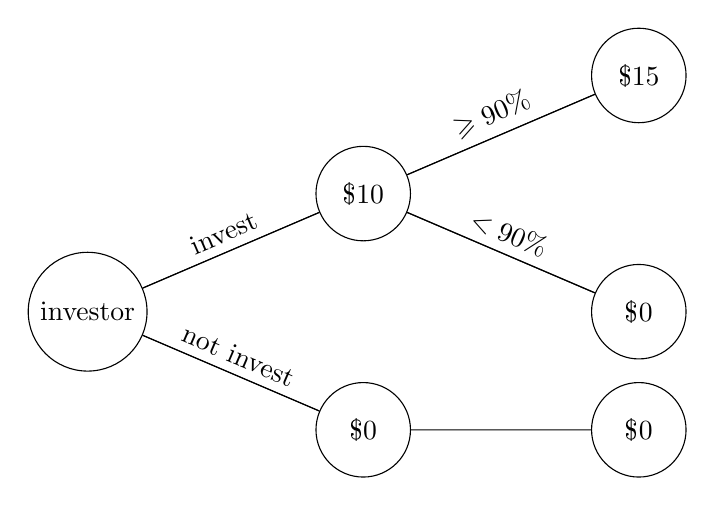
\begin{tikzpicture}
	[
		sloped,grow = 0, sibling distance=3cm, 
		every node/.style = {xshift = 2cm, shape=circle,align=center,draw ,minimum size=1.2cm},
	]
  
  \node (R) {investor}
  	child{
  		node (o) {\$0} 
  		child{ node (O) {\$0}}
  	}
  	child{
  		node (I) {\$10}
  		child {
			node (L) {\$0}
  		}
  		child {
			node (M) {\$15}
  		}
  	};
  	
  \path[every node/.style={},sloped]
  (R) edge node [above] {invest} (I)
  (R) edge node [above] {not invest} (o)
  (I) edge node [above] {$\geqslant 90\%$} (M)
  (I) edge node [above] {$<90\%$} (L);

\end{tikzpicture}
\end{center}


\section{S6.5 battle of sexes}
\begin{center}
\begin{tabular}{c|ccc}
 & B & G & S \\
 \hline
 B & 2,1 & 0,0 & 0,-1 \\
 G & 0,0 & 1,2 & 0,-2 \\
 S & -1,0 & -1,0 & -2,-2 \\
\end{tabular}
\end{center}

\section{S6.20 Cornot Dupoly}
\hspace{\parindent}cost: $cq$

strategy: $q_1$, $q_2$

price: $p = a-b(q_1+q_2)$

payoff:
\[
	f_1 = pq_1 -cq_1 = (a-c)q_1 - bq_1^2 - bq_1q_2
\]
\[
	f_2 = pq_2 -cq_2 = (a-c)q_2 - bq_2^2 - bq_1q_2
\]


\section{S7.3 Betrand competition for price}
\hspace{\parindent}marginal cost: $c$

price strategy: $p_1$, $p_2$, $0\leq p_i \leq 1$

quantitive: \[ Q(p) = 1-p,\quad p=min\{p_1,p_2\}\]

\[
\begin{array}{ll}
q_1 = \left\{ 
\begin{array}{ll}
	1-p_1 & p_1 < p_2 \\
	0 & p_1 > p_2 \\
	1-\frac{p_1}{2} & p_1 = p_2 \\
\end{array} \right . &  q_2 = \left \{ 
\begin{array}{ll}
	1-p_2 & p_2 < p_1 \\
	0 & p_2 > p_1 \\
	1-\frac{p_2}{2} & p_2 = p_1 \\
\end{array} \right . \\
\end{array}
\]

utility functions
\[
f_1 = p_1q_1-cq_1 \quad f_2 = p_2q_2 - cq_2
\]


\section{S7.29 Not identical product}

\begin{center}
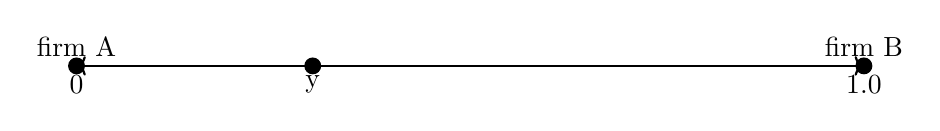
\begin{tikzpicture}
	\draw [thick, <->] (0,0) -- (3,0) -- (10,0);
	\draw [fill] (0,0) circle [radius=0.1];
	\draw [fill] (3,0) circle [radius=0.1];
	\draw [fill] (10,0) circle [radius=0.1];
	\node at (0,0) [above] {firm A};
	\node at (0,0) [below] {0};
	\node at (10,0) [above] {firm B};
	\node at (10,0) [below] {1.0};
	\node at (3,0) [below] {y};
\end{tikzpicture}
\end{center}

y's choice
\[
\mathrm{min}\{p_1+ty^2,p_2+t(1-y)^2\}
\]

\section{S7.42 voting again}

settings:

1. the number of candidates is not fixed.

2. candidates cannot choose their position, their 'born' there.

3. each voter is a potential candidate

4. vote for the closest candidate

5. winner has the most number of votes, if tie, just randomly split the votes.

players: candidates

stragtegy: run or not run

\[
\mathrm{payoff_x} = \left\{ \begin{array}{ll}
-C-|x-y| & x\;run,but\;loss\\
B & x\;run,and\;win\;B \geq 2C \\
-|x-y| & x\;not\;run\;and\;y\; wins\\
\end{array}\right.
\]

\begin{center}
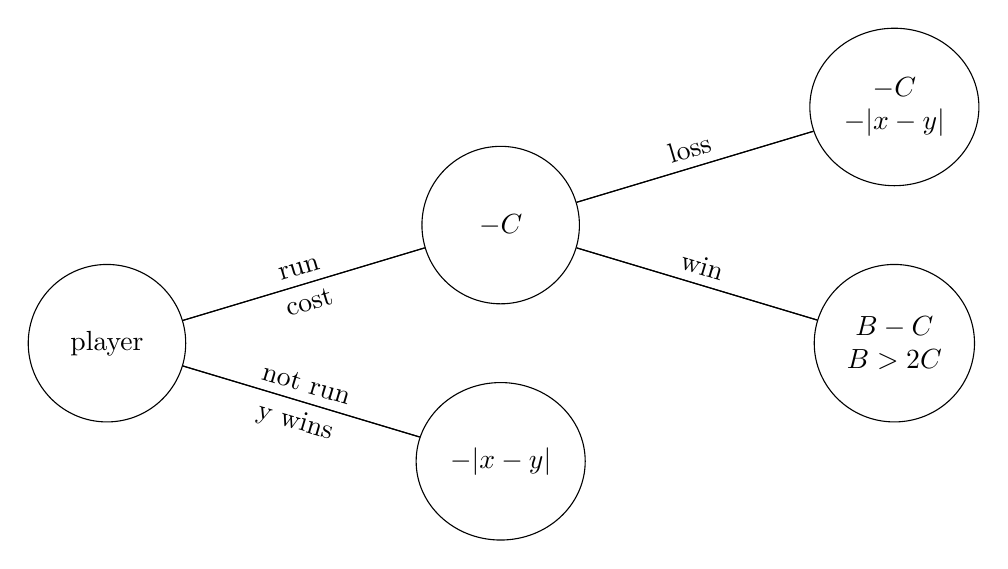
\begin{tikzpicture}
	[
		sloped,grow = 0, sibling distance=3cm, 
		every node/.style = {xshift = 3.5cm, shape=ellipse ,align=center,draw ,minimum size=2cm},
	]
  
  \node (P) {player}
  	child{
  		node (notrun) {$-|x-y|$} 
  	}
  	child{
  		node (run) {$-C$}
  		child {
			node (win) {$B-C$ \\ $B>2C$}
  		}
  		child {
			node (loss) {$-C$ \\ $-|x-y|$}
  		}
  	};
  	
  \path[every node/.style={},sloped]
  (P) edge node [above] {not run} node [below] {y wins} (notrun)
  (P) edge node [above] {run} node [below] {cost}  (run)
  (run) edge node [above] {win} (win)
  (run) edge node [above] {loss} (loss);

\end{tikzpicture}
\end{center}

\section{S8.15 segregating}

which city people will choose to live?

There are two cities E and W. Each has a capacity of 100K residents.

There are two types of people, T and S. Again, there are 100K for each.

the strategy for each people is ${E,W}$.

if over capacity, people will be random to re-located.
\begin{center}
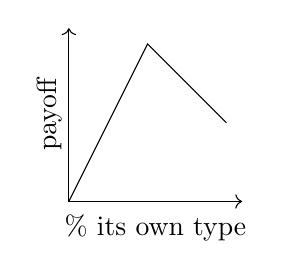
\begin{tikzpicture}
\draw [<->] (0,2.2) -- (0,0) -- (2.2,0);
\node[align=center, below] at (1.1,-.05) {\% its own type};
\node[align=center,rotate = 90] at (-0.25,1.1) {payoff};
\draw (0,0) --(1,2) -- (2,1);
\end{tikzpicture}
\end{center}



\section{S8.1:05 ROCK-PAPER-SCISSORS}
\begin{center}
\begin{tabular}{c|ccc}
 & R & P & S \\
 \hline
 R & 0,0 & -1,1 & 1,-1 \\
 P & 1,-1 & 0,0 & -1,1 \\
 S & -1,1 & 1,-1 & 0,0 \\
\end{tabular}
\end{center}


\section{S9.6 mix strategy}
\begin{center}
\begin{tabular}{c|cc}
 & a & b\\
 \hline
 A & 2,1 & 0,0 \\
 B & 0,0 & 1,2 \\
\end{tabular}
\end{center}

\section{S9.6 strategic effect}
\begin{center}
\begin{tabular}{ccc}
\begin{tabular}{c|cc}
 & l & r\\
 \hline
 L & 50,50 & 80,20 \\
 R & 90,10 & 20,80 \\
\end{tabular} & $\rightarrow$ &
\begin{tabular}{c|cc}
 & l & r\\
 \hline
 L & 30,70 & 80,20 \\
 R & 90,10 & 20,80 \\
\end{tabular}
\end{tabular}
\end{center}



\section{S9.6 tax code}
tax payer = \{H:honest, C: cheat\} , tax auditor = \{A: audit, N: not audit\}
\begin{center}
\begin{tabular}{ccccc}
\begin{tabular}{c|cc}
 & H & C\\
 \hline
 A & 2,0 & 4,-10 \\
 N & 4,0 & 0,4 \\
\end{tabular} & $\rightarrow$ &
\begin{tabular}{c|cc}
 & H & C\\
 \hline
 A & 2,0 & 4,-20 \\
 N & 4,0 & 0,4 \\
\end{tabular} & $\rightarrow$ &
\begin{tabular}{c|cc}
 & H & C\\
 \hline
 A & 2,0 & 4,-20 \\
 N & 4,0 & 0,6 \\
\end{tabular}
\end{tabular}
\end{center}



\section{S11.11 within species competetion}
symmetry 2-player game
random matching 2 players in a population
two types of things in the population: cop and def.

\begin{center}
\begin{tabular}{c|cc}
 & Cop & Def\\
 \hline
 cop & 2,2 & 0,3 \\
 def & 3,0 & 1,1 \\
\end{tabular}
\end{center}


\section{S11.33 invation}
\begin{center}
\begin{tabular}{c|ccc}
 & a & b & c \\
 \hline
 a & 2,2 & 0,0 & 0,0 \\
 b & 0,0 & 0,0 & 1,1 \\
 c & 0,0 & 1,1 & 0,0 \\
\end{tabular}
\end{center}

\section{S11.44 more}
\begin{center}
\begin{tabular}{ccc}
\begin{tabular}{c|cc}
 & a & b\\
 \hline
 a & 1,1 & 0,0 \\
 b & 0,0 & 0,0 \\
\end{tabular} &\begin{tabular}{c|cc}
 & a & b\\
 \hline
 a & 1,1 & 1,1 \\
 b & 1,1 & 0,0 \\
\end{tabular} &\begin{tabular}{c|cc}
 & a & b\\
 \hline
 a & 2,2 & 0,0 \\
 b & 0,0 & 1,1 \\
\end{tabular}

\end{tabular}
\end{center}

\section{S12.10 x-morphic}
\begin{center}
\begin{tabular}{c|cc}
 & a & b\\
 \hline
 a & 0,0 & 2,1 \\
 b & 1,2 & 0,0 \\
\end{tabular}
\end{center}


\section{S12.31 Hawk-Dove}
\[
\begin{array}{c|cc}
 & H & D\\
 \hline
 \\
 H & \displaystyle\frac{V-C}{2},\displaystyle\frac{V-C}{2} & V,0 \\
 \\
 D & 0,V & \displaystyle\frac{V}{2},\displaystyle\frac{V}{2}\\
\end{array}
\]


\section{S12.60 cycling pattern}
\[
\begin{array}{c|ccc}
 & S & B & T\\
 \hline
 S & 1,1 & V,0 & 0,V \\
 B & 0,V & 1,1 & V,0 \\
 T & V,0 & 0,V & 1,1 \\
\end{array}
\quad(1 < V < 2)
\]


\section{S13.0 cash in a hat}
something like invenstment

\[\mathrm{player1} \rightarrow \mathrm{put \$0, \$1, \$3 in a hat.}\]

 \[\mathrm{player2} \rightarrow \left\{ \begin{array}{cl}
1 & \mathrm{match player 1} \\
\\
2 & \mathrm{take the money away} \\
\end{array}\right.
\]

payoff:
\[ 
\text{player 1:} \left\{
\begin{array}{ccl}
0 & \rightarrow & 0 \\
1 & \rightarrow & \left\{\begin{array}{cl}
		1 & \text{if player2 matched} \\
		-1 & \text{if player2 take away}\\
	\end{array} \right.\\
3 & \rightarrow & \left\{\begin{array}{cl}
		3 & \text{if player2 matched} \\
		-3 & \text{if player2 take away}\\
	\end{array} \right.\\
\end{array}
\right.
\]

\[  \mathrm{player 2:} \left\{
\begin{array}{ccl}
\text{take} & \rightarrow &\left\{ \begin{array}{cl}
		1 & \text{if player 1 put \$1} \\
		3 & \text{if player 1 put \$3}\\
	\end{array} \right.\\
\text{match} & \rightarrow & \left\{ \begin{array}{cl}
		1.5 & \text{if player 1 put \$1} \\
		2 & \text{if player 1 put \$3}\\
	\end{array} \right.\\
\end{array}
\right.
\] 



\begin{center}
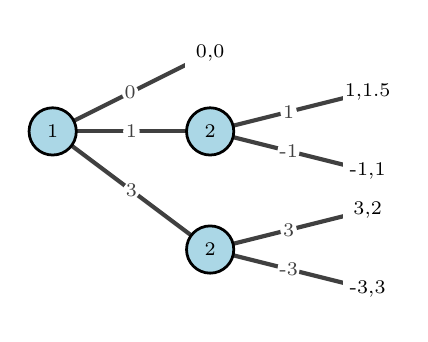
\begin{tikzpicture}
\Vertex[label = 1]{P}
\Vertex[x=2,y=1, shape = rectangle, style = {color = white}, label = {0,0}]{n10}

\Vertex[x=2,label = 2]{n11}
\Vertex[x=4,y=0.5, shape = rectangle, style = {color = white},label = {1,1.5}]{n1211}
\Vertex[x=4,y=-0.5, shape = rectangle, style = {color = white},label = {-1,1}]{n0211}

\Vertex[x=2,y = -1.5,label = 2]{n31}
\Vertex[x=4,y=-1, shape = rectangle, style = {color = white},label = {3,2}]{n3231}
\Vertex[x=4,y=-2, shape = rectangle, style = {color = white},label = {-3,3}]{n0231}

\Edge[label = 0](P)(n10)
\Edge[label = 1](P)(n11)
\Edge[label = 3](P)(n31)
\Edge[label = 1](n11)(n1211)
\Edge[label = -1](n11)(n0211)
\Edge[label = 3](n31)(n3231)
\Edge[label = -3](n31)(n0231)

\end{tikzpicture}
\end{center}


\section{S13.51 norman conquest}

\begin{center}
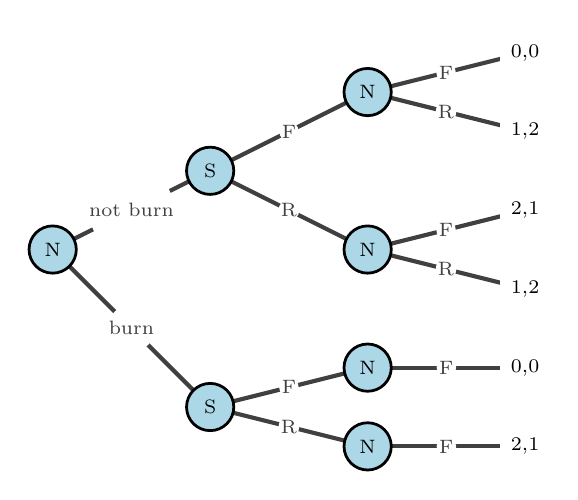
\begin{tikzpicture}
\Vertex[label = N]{P}

\Vertex[x=2,y = 1,label = S]{n21}
\Vertex[x=4,y = 2,label = N]{n31}
	\Vertex[x=6,y = 2.5,shape = rectangle, style = {color = white},label = {0,0}]{n41}
	\Vertex[x=6,y = 1.5,shape = rectangle, style = {color = white},label = {1,2}]{n42}

\Vertex[x=4,y = 0,label = N]{n32}
	\Vertex[x=6,y = 0.5,shape = rectangle, style = {color = white},label = {2,1}]{n43}
	\Vertex[x=6,y = -0.5,shape = rectangle, style = {color = white},label = {1,2}]{n44}
%\Vertex[x=4,y=0.5, shape = rectangle, style = {color = white},label = {1,1.5}]{n1211}

\Vertex[x=2,y = -2,label = S]{n22}
	\Vertex[x=4,y = -1.5,label = N]{n33}
	\Vertex[x=6,y = -1.5,shape = rectangle, style = {color = white},label = {0,0}]{n45}
	\Vertex[x=4,y = -2.5,label = N]{n34}
	\Vertex[x=6,y = -2.5,shape = rectangle, style = {color = white},label = {2,1}]{n46}

\Edge[label=not burn](P)(n21)
\Edge[label=burn](P)(n22)
\Edge[label=F](n21)(n31)
\Edge[label=R](n21)(n32)
\Edge[label=F](n22)(n33)
\Edge[label=R](n22)(n34)

\Edge[label=F](n31)(n41)
\Edge[label=R](n31)(n42)

\Edge[label=F](n32)(n43)
\Edge[label=R](n32)(n44)

\Edge[label=F](n33)(n45)
\Edge[label=F](n34)(n46)

\end{tikzpicture}
\end{center}


\section{S13.1:05 hungry lions}
should lion 1 eat the sheep

\begin{itemize}
\item only lion 1 can eat the sheep
\item lion n+1 can eat lion n
\end{itemize}


\begin{center}
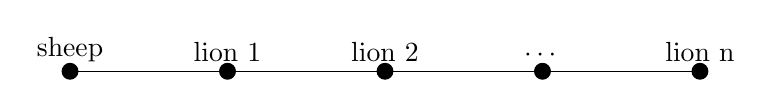
\begin{tikzpicture}
\draw (0,0) node[above]{sheep} -- (2,0) node[above]{lion 1} --(4,0) node[above]{lion 2} -- (6,0) node[above] {$\cdots$} --(8,0) node[above]{lion n};
\draw [fill] (0,0) circle [radius=0.1];
\draw [fill] (2,0) circle [radius=0.1];
\draw [fill] (4,0) circle [radius=0.1];
\draw [fill] (6,0) circle [radius=0.1];
\draw [fill] (8,0) circle [radius=0.1];

\end{tikzpicture}
\end{center}

\section{S14.1 sequential cornot }
\[
p = a - b(q_1+q_2)
\]
\[
f_i = pq_i - cq_i
\]

firm 1 choose $q_1$ first, then firm 2 choose $q_2$ responding to $q_1$.

\section{S14.56 nil: first/second mover advantage}
setting:

two piles of stone, the player need to choose how many stone to remove from one of the stone pile. the who get the last stone wins.

\section{S15.32 stone grid}
setting:

one pile of stone, the player need to choose which stone to remove. And anything on the northwest of the removed stone will also be removed.
the who get the last stone loss.


\section{S15.47 silly equilibrium}
\begin{center}
\begin{tabular}{lc}
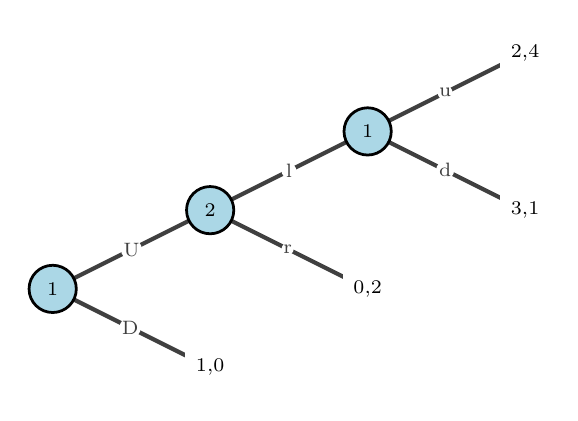
\begin{tikzpicture}
%\newcommand{\leaf}{shape = rectangle,style = {color = white}}

\Vertex[x = 0, y = 1,label = 1]{n1}
\Vertex[x = 2, y = 2,label = 2]{n1u}
\Vertex[x = 2, y = 0,shape = rectangle,style = {color = white}, label = {1,0}]{n1d}
\Vertex[x = 4, y = 3, label = 1]{n1u2l}
\Vertex[x = 4, y = 1, shape = rectangle,style = {color = white},label = {0,2}]{n1u2r}
\Vertex[x = 6, y = 4, shape = rectangle,style = {color = white},label = {2,4}]{n1u2l1u}
\Vertex[x = 6, y = 2, shape = rectangle,style = {color = white},label = {3,1}]{n1u2l1d}

\Edge[label=U](n1)(n1u)
\Edge[label=D](n1)(n1d)
\Edge[label=l](n1u)(n1u2l)
\Edge[label=r](n1u)(n1u2r)
\Edge[label=u](n1u2l)(n1u2l1u)
\Edge[label=d](n1u2l)(n1u2l1d)

\end{tikzpicture} & \begin{tabular}{c|cc}
 & l & r\\
 \hline
 Uu & 2,4 & 0,2 \\
 Ud & 3,1 & 0,2 \\
 Du & 1,0 & 1,0 \\
 Dd & 1,0 & 1,0 \\
\end{tabular}
\end{tabular}

\end{center}

\section{S15.1:02 market invasion}
\begin{center}
\begin{tabular}{lc}
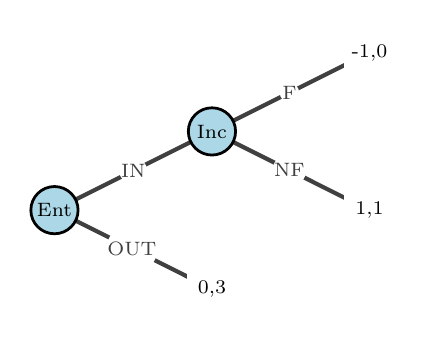
\begin{tikzpicture}

\Vertex[x = 0, y = 1, label = Ent]{n1}
\Vertex[x = 2, y = 0, label = {0,3},shape = rectangle,style = {color = white}]{n1o}
\Vertex[x=2,y=2, label = Inc]{n1i}
\Vertex[x = 4, y= 3, label = {-1,0},shape = rectangle,style = {color = white}]{n1i2f}
\Vertex[x = 4, y= 1, label = {1,1},shape = rectangle,style = {color = white}]{n1i2n}

\Edge[label = IN](n1)(n1i)
\Edge[label = OUT](n1)(n1o)
\Edge[label = F](n1i)(n1i2f)
\Edge[label = NF](n1i)(n1i2n)


\end{tikzpicture} & \begin{tabular}{c|cc}
 & F & NF\\
 \hline
In & -1,0 & 1,1 \\
Out & 0,3 & 0,3 \\
\end{tabular} \\
\end{tabular}

\end{center}

\section{S16.26 Duel}
settings

two player is about to shoot each other. each round the player can choose between shotting, if the ball is avable, or step forward.


\section{S17.01 ultimatum}
setting
\$1 on the table

player 1 make an offer to player 2 with $0<x<\$1$, while keep the rest.

player 2 can accpet or reject the offer.

\noindent payoff

player 2 accpet $\rightarrow (1-x,x)$

player 2 reject $\rightarrow (0,0)$

\section{S17.14 two period bargaining game to infinite bargaining}
\noindent stage 1:

\$1 on the table

player 1 make an offer to player 2 with $0<x<\$1$, while keep the rest.

if player 2 accpet the offer  $\rightarrow (1-x,x)$

if player 2 reject, flip the role and move to stage 2

\noindent stage 2:

the \$1 on the table is shrink to $\$\delta$

player 2 make an offer to player 1 with $0<x<\$\delta$, while keep the rest.

if player 1 accpet the offer  $\rightarrow (\$\delta-x,x)$

if player 1 reject $(0,0)$


\section{S18.02 information set}
\begin{tabular}{lr}
\begin{tikzpicture}
[grow = 0,level distance=30mm]
\tikzset{
	player1/.style = {circle, draw, inner sep = 1.5, label = below:{p1}},
	player2/.style = {circle, draw, inner sep = 1.5,fill = black,label = below:{p2}},
	level 1/.style = {sibling distance=30mm},
	level 2/.style = {sibling distance=22mm}
}

\node(0) [player1]{}
	child{
		node [player2]{}
		child{
			node {0,0}
			edge from parent node [circle,fill=white]{\footnotesize r}
		}
		child{
			node {1,2}
			edge from parent node [circle,fill=white]{\footnotesize l}
		}
			edge from parent node [circle,fill=white]{\footnotesize D}
	}
	child{
		node [player2]{}
		child{
			node{4,0}
			edge from parent node [circle,fill=white]{\footnotesize d}			
		}
		child{
			node{0,4}
			edge from parent node [circle,fill=white]{\footnotesize u}		
		}
			edge from parent node [circle,fill=white]{\footnotesize M}
	}
	child{
		node [player2]{}
		child{
			node {0,4}
			edge from parent node [circle,fill=white]{\footnotesize d}			
		}
		child{
			node{4,0}
			edge from parent node [circle,fill=white]{\footnotesize u}					
		}
			edge from parent node [circle,fill=white]{\footnotesize U}		
	}	
;

\end{tikzpicture} & \begin{tikzpicture}
[grow = 0,level distance=30mm]
\tikzset{
	player1/.style = {circle, draw, inner sep = 1.5, label = below:{p1}},
	player2/.style = {circle, draw, inner sep = 1.5,fill = black,label = below:{p2}},
	level 1/.style = {sibling distance=30mm},
	level 2/.style = {sibling distance=22mm}
}

\node(0) [player1]{}
	child{
		node [player2]{}
		child{
			node {0,0}
			edge from parent node [circle,fill=white]{\footnotesize r}
		}
		child{
			node {1,2}
			edge from parent node [circle,fill=white]{\footnotesize l}
		}
			edge from parent node [circle,fill=white]{\footnotesize D}
	}
	child{
		node [player2]{}
		child{
			node{4,0}
			edge from parent node [circle,fill=white]{\footnotesize d}			
		}
		child{
			node{0,4}
			edge from parent node [circle,fill=white]{\footnotesize u}		
		}
			edge from parent node [circle,fill=white]{\footnotesize M}
	}
	child{
		node [player2]{}
		child{
			node {0,4}
			edge from parent node [circle,fill=white]{\footnotesize d}			
		}
		child{
			node{4,0}
			edge from parent node [circle,fill=white]{\footnotesize u}					
		}
			edge from parent node [circle,fill=white]{\footnotesize U}		
	}	
;

\draw [dashed] (0-2) to (0-3);
\end{tikzpicture} \\
\end{tabular}


\section{S18.19 prisoner's dilemma in tree}
\begin{center}
\begin{tikzpicture}
[grow = 0,level distance=30mm]
\tikzset{
	player1/.style = {circle, draw, inner sep = 1.5, label = below:{p1}},
	player2/.style = {circle, draw, inner sep = 1.5,fill = black,label = below:{p2}},
	level 1/.style = {sibling distance=30mm},
	level 2/.style = {sibling distance=22mm}
}

\node(0) [player1]{}
	child{
		node [player2]{}
		child{
			node {0,0}
			edge from parent node [circle,fill=white]{\footnotesize r}
		}
		child{
			node {3,-1}
			edge from parent node [circle,fill=white]{\footnotesize l}
		}
			edge from parent node [circle,fill=white]{\footnotesize D}
	}
	child{
		node [player2]{}
		child{
			node{-1,3}
			edge from parent node [circle,fill=white]{\footnotesize r}			
		}
		child{
			node{2,2}
			edge from parent node [circle,fill=white]{\footnotesize l}		
		}
			edge from parent node [circle,fill=white]{\footnotesize U}
	}
;

\draw [dashed] (0-1) to (0-2);
\end{tikzpicture}
\end{center}

\section{S18.29 transpose}
\begin{tabular}{cc}
\begin{tikzpicture}
[grow = 0,level distance=30mm]
\tikzset{
	player1/.style = {circle, draw, inner sep = 1.5, label = below:{p1}},
	player2/.style = {circle, draw, inner sep = 1.5,fill = black,label = below:{p2}},
	level 1/.style = {sibling distance=43mm},
	level 2/.style = {sibling distance=18mm}
}

\node(0) [player1]{}
	child{
		node [player2]{}
		child{
			node {$f_1,f_2$}		
			edge from parent node [circle,fill=white]{\footnotesize r}
		}
		child{
			node {$e_1,e_2$}
			edge from parent node [circle,fill=white]{\footnotesize c}			
		}
		child{
			node {$d_1,d_2$}
			edge from parent node [circle,fill=white]{\footnotesize l}			
		}
		edge from parent node [circle,fill=white]{\footnotesize D}
	}
	child{
		node [player2]{}
		child{
			node {$c_1,c_2$}
			edge from parent node [circle,fill=white]{\footnotesize r}
		}
		child{
			node {$b_1,b_2$}
			edge from parent node [circle,fill=white]{\footnotesize c}			
		}
		child{
			node {$a_1,a_2$}
			edge from parent node [circle,fill=white]{\footnotesize l}			
		}
		edge from parent node [circle,fill=white]{\footnotesize U}
	}
;

\draw [dashed] (0-1) to (0-2);


\end{tikzpicture} & \begin{tikzpicture}
[grow = 0,level distance=30mm]
\tikzset{
	player1/.style = {circle, draw, inner sep = 1.5, label = below:{p1}},
	player2/.style = {circle, draw, inner sep = 1.5,fill = black,label = below:{p2}},
	level 1/.style = {sibling distance=30mm},
	level 2/.style = {sibling distance=20mm}
}

\node(0) [player2]{}
	child{
		node [player1]{}
		child{
			node {$f_1,f_2$}
			edge from parent node [circle,fill=white]{\footnotesize D}	
		}
		child{
			node {$c_1,c_2$}
			edge from parent node [circle,fill=white]{\footnotesize U}				
		}
		edge from parent node [circle,fill=white]{\footnotesize r}		
	}		
	child{
		node [player1]{}
		child{
			node {$e_1,e_2$}
			edge from parent node [circle,fill=white]{\footnotesize D}	
		}
		child{
			node {$b_1,b_2$}
			edge from parent node [circle,fill=white]{\footnotesize U}				
		}
		edge from parent node [circle,fill=white]{\footnotesize c}					
	}
	child{
		node [player1]{}
		child{
			node {$d_1,d_2$}
			edge from parent node [circle,fill=white]{\footnotesize D}	
		}
		child{
			node {$a_1,a_2$}
			edge from parent node [circle,fill=white]{\footnotesize U}				
		}
		edge from parent node [circle,fill=white]{\footnotesize l}		
	}
;

\draw [dashed] (0-1) to (0-2) to (0-3);


\end{tikzpicture}

\end{tabular}

\section{S18.35 }
\begin{center}
\begin{tikzpicture}
[grow = 0,level distance=30mm]
\tikzset{
	player1/.style = {circle, draw, inner sep = 1.5, label = below:{p1}},
	player2/.style = {circle, draw, inner sep = 1.5,fill = black,label = below:{p2}},
	level 1/.style = {sibling distance=37mm},
	level 2/.style = {sibling distance=20mm},
	level 3/.style = {sibling distance=20mm}
}

\node(0) [player1]{}
	child{
		node [player2]{}
		child{
			node {2,4}
			edge from parent node [circle,fill=white]{\footnotesize r}
		}
		child{
			node {0,0}
			edge from parent node [circle,fill=white]{\footnotesize l}
		}
			edge from parent node [circle,fill=white]{\footnotesize D}
	}
	child{
		node [player2]{}
		child{
			node [player1]{}
			child{
				node {1,4}
				edge from parent node [circle,fill=white]{\footnotesize d}				
			}
			child{
				node {0,0}
				edge from parent node [circle,fill=white]{\footnotesize u}				
			}
			edge from parent node [circle,fill=white]{\footnotesize r}		
		}
		child{
			node{4,2}
			edge from parent node [circle,fill=white]{\footnotesize l}			
		}
			edge from parent node [circle,fill=white]{\footnotesize U}
	}
;

\draw [dashed] (0-1) to (0-2);
\end{tikzpicture}
\end{center}

\section{S18.50 }
\begin{center}
\begin{tikzpicture}
[grow = 0,level distance=30mm]
\tikzset{
	player1/.style = {circle, draw, inner sep = 1.5,fill = red, label = below:{p1}},
	player2/.style = {circle, draw, inner sep = 1.5,fill = white,label = below:{p2}},
	player3/.style = {circle, draw, inner sep = 1.5,fill = black,label = below:{p3}},
	payoff/.style ={circle,draw,inner sep = 1.5},
	level 1/.style = {sibling distance=30mm},
	level 2/.style = {sibling distance=30mm},
	level 3/.style = {sibling distance=25mm}
}

\node(0) [player1]{}
	child{
		node [player2]{}
		child{
			node[player3]{}
			child{
				node {2,1,0}
				edge from parent node [circle,fill=white]{\footnotesize r}				
			}
			child{
				node {0,0,-1}			
				edge from parent node [circle,fill=white]{\footnotesize l}
			}
			edge from parent node [circle,fill=white]{\footnotesize D}
		}
		child{
			node[player3]{}
			child{
				node {0,0,2}
				edge from parent node [circle,fill=white]{\footnotesize r}
			}
			child{
				node{0,1,1}
				edge from parent node [circle,fill=white]{\footnotesize l}
			}
			edge from parent node [circle,fill=white]{\footnotesize U}
		}
		edge from parent node [circle,fill=white]{\footnotesize B}
	}
	child{
		node {1,0,0}
		edge from parent node [circle,fill=white]{\footnotesize A}
	}
;

\draw [dashed] (0-1-1) to (0-1-2);
\end{tikzpicture}
\end{center}



\section{S19.01 don't screw up}
\begin{center}
\begin{tikzpicture}
[grow = 0,level distance=30mm]
\tikzset{
	player1/.style = {circle, draw, inner sep = 1.5,fill = white, label = below:{p1}},
	player2/.style = {circle, draw, inner sep = 1.5,fill = black,label = below:{p2}},
	payoff/.style ={circle,draw,inner sep = 1.5},
	level 1/.style = {sibling distance=30mm},
	level 2/.style = {sibling distance=30mm},
	level 3/.style = {sibling distance=25mm}
}

\node(0) [player1]{}
	child{
		node {2,1}
		edge from parent node [circle,fill=white]{\footnotesize D}	
	}
	child{
		node [player2]{}
		child{
			node{1,2}
			edge from parent node [circle,fill=white]{\footnotesize r}			
		}
		child{
			node [player1]{}
			child{
				node{3,1}
				edge from parent node [circle,fill=white]{\footnotesize d}				
			}
			child{
				node{4,3}
				edge from parent node [circle,fill=white]{\footnotesize u}	
			}
			edge from parent node [circle,fill=white]{\footnotesize l}						
		}
		edge from parent node [circle,fill=white]{\footnotesize U}
	}
;

\end{tikzpicture}
\end{center}




\section{S19.30 matchmaker}
\begin{center}
\begin{tikzpicture}
[grow = 0,level distance=30mm]
\tikzset{
	player1/.style = {circle, draw, inner sep = 1.5,fill = red, label = below:{p1}},
	player2/.style = {circle, draw, inner sep = 1.5,fill = white,label = below:{p2}},
	player3/.style = {circle, draw, inner sep = 1.5,fill = black,label = below:{p3}},
	payoff/.style ={circle,draw,inner sep = 1.5},
	level 1/.style = {sibling distance=30mm},
	level 2/.style = {sibling distance=30mm},
	level 3/.style = {sibling distance=25mm}
}

\node(0) [player1]{}
	child{
		node [player2]{}
		child{
			node[player3]{}
			child{
				node {1,1,2}
				edge from parent node [circle,fill=white]{\footnotesize S}				
			}
			child{
				node {-1,0,0}			
				edge from parent node [circle,fill=white]{\footnotesize G}
			}
			edge from parent node [circle,fill=white]{\footnotesize S}
		}
		child{
			node[player3]{}
			child{
				node {-1,0,0}
				edge from parent node [circle,fill=white]{\footnotesize S}
			}
			child{
				node{1,2,1}
				edge from parent node [circle,fill=white]{\footnotesize G}
			}
			edge from parent node [circle,fill=white]{\footnotesize G}
		}
		edge from parent [draw= none]
	}
	child{
		node {0,0,0}
		edge from parent [draw= none]
	}
;

\path[every node/.style={},sloped]
 (0) edge node [above] {not send} (0-2)
 (0) edge node [below] {send} (0-1)
 ;


\draw [dashed] (0-1-1) to (0-1-2);
\end{tikzpicture}
\end{center}

\section{S19.50 strategic investment}
two firms intially are playing cournot.
\[
	p = 2-\frac{1}{3}(q_A+q_B)
\]

\noindent cost: $c=1$ per ton.

\[
	\mathrm{quantity:}\; q^c = \frac{a-c}{3b} = \frac{2-1}{3\times 1/3} = 1
\]

\[
	\mathrm{price:}\; p = 2- 2/3 = \frac{4}{3}
\]

\[
	\mathrm{profit} = (p-c)\times q^c = \frac{1}{3}
\]

\noindent firm A need to make decision to rent or not a new machine:

rental: $c_0 = 0.7$

reduce cost to: $c = 0.5$

\section{S20.02 fight or quit}
2 players

each choose fight or quit

the game ends if some one quit

\noindent payoff and cost

\vspace{0.5cm}

\begin{tabular}{c|cc}
 & fight & quit\\
 \hline
 F & -c,-c & v,0 \\
 Q & 0,v & 0,0 \\
\end{tabular}

\vspace{0.5cm}

\noindent note: if keep fighting, the game can last forever.

\section{S20.28 Wars of Attrition}

assume: $v>c$

one period game

\begin{tikzpicture}
[grow = 0,level distance=30mm]
\tikzset{
	player1/.style = {circle, draw, inner sep = 1.5, label = below:{p1}},
	player2/.style = {circle, draw, inner sep = 1.5,fill = black,label = below:{p2}},
	level 1/.style = {sibling distance=30mm},
	level 2/.style = {sibling distance=22mm}
}

\node(0) [player1]{}
	child{
		node [player2]{}
		child{
			node {0,0}
			edge from parent node [circle,fill=white]{\footnotesize q}
		}
		child{
			node {0,v}
			edge from parent node [circle,fill=white]{\footnotesize f}
		}
			edge from parent node [circle,fill=white]{\footnotesize Q}
	}
	child{
		node [player2]{}
		child{
			node{v,0}
			edge from parent node [circle,fill=white]{\footnotesize q}			
		}
		child{
			node{-c,-c}
			edge from parent node [circle,fill=white]{\footnotesize f}		
		}
			edge from parent node [circle,fill=white]{\footnotesize F}
	}
;

\draw [dashed] (0-1) to (0-2);
\end{tikzpicture}

two period game

\begin{tikzpicture}
[grow = 0,level distance=30mm]
\tikzset{
	player1/.style = {circle, draw, inner sep = 1.5, label = below:{p1}},
	player2/.style = {circle, draw, inner sep = 1.5,fill = black,label = below:{p2}},
	level 1/.style = {sibling distance=30mm},
	level 2/.style = {sibling distance=22mm},
	level 3/.style = {sibling distance=30mm},
	level 4/.style = {sibling distance=22mm}
}

\node(0) [player1]{}
	child{
		node [player2]{}
		child{
			node {0,0}
			edge from parent node [circle,fill=white]{\footnotesize q}
		}
		child{
			node {0,v}
			edge from parent node [circle,fill=white]{\footnotesize f}
		}
			edge from parent node [circle,fill=white]{\footnotesize Q}
	}
	child{
		node [player2]{}
		child{
			node{v,0}
			edge from parent node [circle,fill=white]{\footnotesize q}			
		}
		child{
			node [player1]{}
			child{
		node [player2]{}
		child{
			node {-c+0,-c+0}
			edge from parent node [circle,fill=white]{\footnotesize q}
		}
		child{
			node {-c+0,-c+v}
			edge from parent node [circle,fill=white]{\footnotesize f}
		}
			edge from parent node [circle,fill=white]{\footnotesize Q}
	}
	child{
		node [player2]{}
		child{
			node{-c+v,-c+0}
			edge from parent node [circle,fill=white]{\footnotesize q}			
		}
		child{
			node{-c-c,-c-c}
			edge from parent node [circle,fill=white]{\footnotesize f}		
		}
			edge from parent node [circle,fill=white]{\footnotesize F}
	}
			edge from parent node [circle,fill=white]{\footnotesize f}		
		}
			edge from parent node [circle,fill=white]{\footnotesize F}
	}
;

\draw [dashed] (0-1) to (0-2);
\draw [dashed] (0-2-2-1) to (0-2-2-2);
\end{tikzpicture}

\section{S21.06 repeated prisoner's dilemma: grim trigger}
\begin{tabular}{c|cc}
 & corp & defe \\
 \hline
 corp & 2,2 & -1,3 \\
 defe & 3,-1 & 0,0 \\
\end{tabular}

\vspace{0.5cm}
\noindent how to end:
\begin{itemize}
\item two period, three period
\item toss a coin twice, HH ends
\end{itemize}

\section{S21.22 repeated altered prisoner's dilemma}
\begin{tabular}{c|ccc}
 & a & b & c\\
 \hline
 a & 4,4 & 0,5 & 0,0 \\
 b & 5,0 & 1,1 & 0,0 \\
 c & 0,0 & 0,0 & 3,3 \\
\end{tabular}

\vspace{0.5cm}
\noindent use (b,b) as a punishment. use (c,c) as reward.

\section{S22.01 repeated prisoner's dilemma:discounting tomorrow or probability of continous}
\begin{tabular}{c|cc}
 & corp & defe \\
 \hline
 corp & 2,2 & -1,3 \\
 defe & 3,-1 & 0,0 \\
\end{tabular}

\vspace{0.5cm}
\noindent corp condition

\[
	3-2 \le \delta(2+2\delta + 2\delta^2+\cdots - 0)
\]

\section{S22.53 repeated moral hazard}

\begin{center}
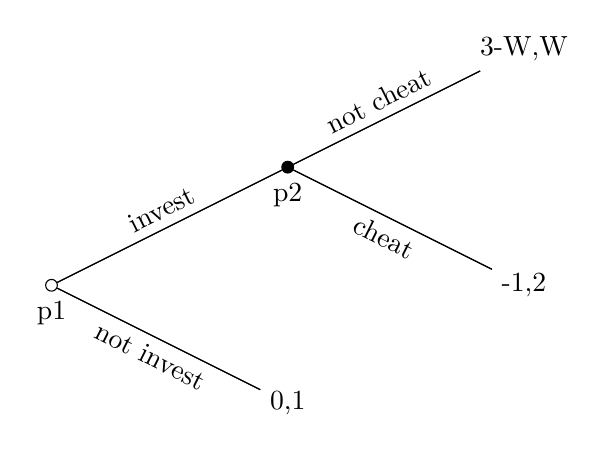
\begin{tikzpicture}
[grow = 0,level distance=30mm]
\tikzset{
	player1/.style = {circle, draw, inner sep = 1.5, label = below:{p1}},
	player2/.style = {circle, draw, inner sep = 1.5,fill = black,label = below:{p2}},
	level 1/.style = {sibling distance=30mm},
	level 2/.style = {sibling distance=30mm}
}

\node(0) [player1]{}
	child{
		node {0,1}	
	}
	child{
		node [player2] {}
		child{
			node {-1,2}
		}
		child{
			node {3-W,W}
		}
	}
;


\path[every node/.style={},sloped]
	(0) edge node [below] {not invest} (0-1)
	(0) edge node [above] {invest} (0-2)
	(0-2) edge node [below] {cheat} (0-2-1)
	(0-2) edge node [above] {not cheat} (0-2-2)
	;

\end{tikzpicture}
\end{center}

\vspace{0.5cm}
probability to repeat $\delta$, what wage should you pay?



\section{S23.00 Revealing your costs in Cournot}

firm B has cost $c_m$,

\noindent firm A has cost:
\[
c = \left\{\begin{array}{l}
c_h = c_m +x \\
c_m \\
c_l = c_m -x 
\end{array}
\right.
\]

should you reveal your costs?

\section{S23.51 Spence Education-Signaling}
two types of works:

good works and bad works

effeciency: 50 vs. 30

popultation: 10\% vs. 90\%

\noindent firms compete for works, pay 50 to workers label as good, while pay 30 to workers as bad, pay 32 to unknown workers.

\noindent how to signal that you are a good workers?

the cost of getting MBA for good worker is 5 per year.

the cost of getting MBA for bad worker is 10 per year.

the degree take 3 years, and the firms identify MBA as good, no MBA as bad.

\noindent the players are the firms, good workers, bad workers.

\section{S24.01 Auctions}
common value auction, goods can be re-sell.

guess how much money in the jar, and place a bid.

bid the estimate vs. shave the estimate a bit.

why we fall into the "winner's curse".

reason 1. the winner is the one with the biggest error, instead of the closest estimate.

how to minimazed your regret. bid as if you know you win.

\vspace{0.5cm}

\noindent imagine:  \textbf{you have won (which means your bid is the highest), and you were given another chance to estimate again. that estimate should be the bid.}

\vspace{0.5cm}
\begin{itemize}
\item first price bid seal auction.
\item second price bid seal auction.
\item ascending open auction.
\item descending open auction.
\end{itemize}

in private value auction, no need to consider about re-selling.

in second price auction, the bid should be your value.

in first price auction, the bid should be less than your value.

from the seller point of view, which auction can generate more revenue?

\end{document}
